\documentclass{oblivoir}
    \usepackage{ikps} %일격필살에서 배포한 패키지
    \usepackage{hyperref}
    \usepackage{graphicx}


\begin{document}

\title{simple report}
\author{이윤승 201712052}
\maketitle
\tableofcontents

\secton{Vitual memory}
컴퓨터를 켜면 많은 프로그램이 돌아가고있다. 이 프로그램의 메모리관리를
하드웨어 단위로 했을때 서로 다른 프로그램의 자료를 덮어쓰는 문제 등이 발생에
관리에 어려움이 있기에 충동을 막기위해 OS에서는 각 프로그램에 가상메모리를 제공하고 OS에서 직접
하드웨어에 메모리 할당을 자동으로 해주는 식으로 한다. \textbf{MMU(Memory Mangement Unit)}는 
CPU가 메모리에 접근하는 것을 관리하는 하드웨어 부품이다.
\begin{figure}[h!]
    \centering
    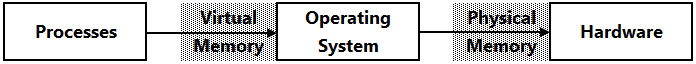
\includegraphics[scale = 0.5]{virtual_memory.png}
\end{figure}
\begin{figure}[h!]
    \centering
    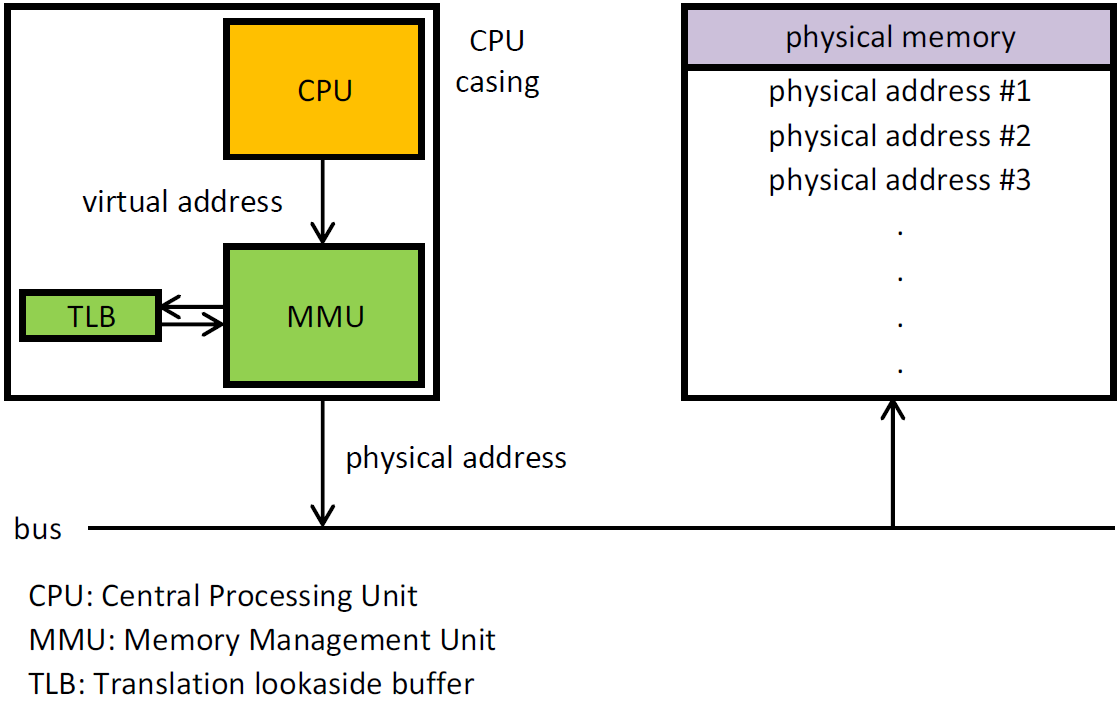
\includegraphics[scale = 0.5]{MMU.png}
\end{figure}
이 가상 메모리의 크기는 실제 메모리의 크기보다 크게 설정을 해서 할수도있다.
메모리 할당은 주기억장치에 주로 램을 사용하고,램에서 잘 쓰지는 않는 데이터는 보조기억장치로서 하드디스크(and SSD)에 저장해서 관리한다.
이때 보조기억장치는 램에비해서 매우 느리니 유의할것.
\url{https://answers.microsoft.com/en-us/windows/forum/windows_10-performance/physical-and-virtual-memory-in-windows-10/e36fb5bc-9ac8-49af-951c-e7d39b979938}
너무 어려워요 ㅠㅠ









\section{Stack frame}
\textbf{콜스택}\\
컴퓨터 프로그램에서 스택 데이터 구조 

콜스택에서 함수등을 부를 때 스택에 들어가는 정보들을 스택프레임이라 한다.
해당하는 프로세스가 실행중일때만 존재하고 사라진다. 이를 이용해서 recursion을 구현할수있다.

\begin{figure}[h!]
    \centering
    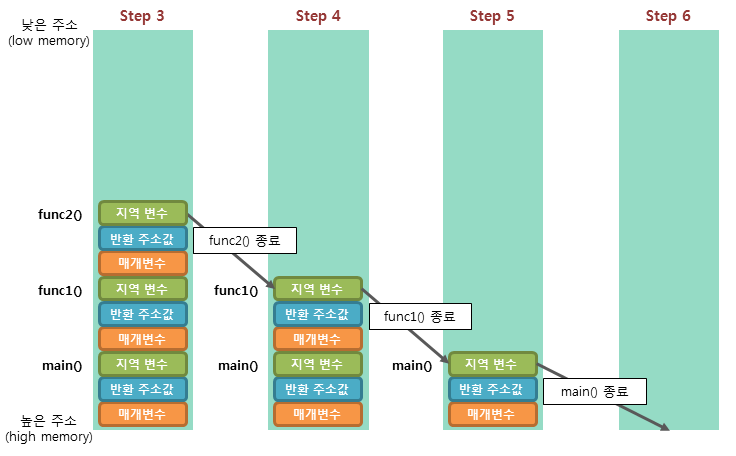
\includegraphics[scale = 0.5]{stackframe.png}
\end{figure}
함수의 콜스택에서 들어가는 정보들.
\begin{itemize}
    \item 현재상태의 포인터
    \item parameter
    \item 로컬 데이터 저장소(local data storage)
    \item 다른 반환 상태(other return state)
\end{itemize}


\section{참고, 출처}

\url{https://answers.microsoft.com/en-us/windows/forum/windows_10-performance/physical-and-virtual-memory-in-windows-10/e36fb5bc-9ac8-49af-951c-e7d39b979938} 
\\ \url{http://tcpschool.com/c/c_memory_stackframe}
\\ \url{https://www.techopedia.com/definition/22304/stack-frame}
\\ \url{http://tcpschool.com/c/c_memory_stackframe}
\\ \url{https://stackoverflow.com/questions/10057443/explain-the-concept-of-a-stack-frame-in-a-nutshell}
\\ \url{https://en.wikipedia.org/wiki/Call_stack}
\\ \url{https://ko.wikipedia.org/wiki/%EA%B0%80%EC%83%81_%EB%A9%94%EB%AA%A8%EB%A6%AC}
\\ \url{https://namu.wiki/w/%EA%B0%80%EC%83%81%EB%A9%94%EB%AA%A8%EB%A6%AC}
\\ \url{}
\end{document}